%!TEX program = xelatex

\documentclass[cn,black,9pt,normal]{elegantnote}
\usepackage{float}
\usepackage{hyperref}


%\newcommand{\upcite}[1]{\textsuperscript{\textsuperscript{\cite{#1}}}}

\title{数码摄影作业(08)色彩\\\small{实验室准入卡}}
\author{姓名:姜文渊\\学号:1951510}
%\institute{School of Life Science, Tongji University}
%\version{1.00}
\date{2021年4月25日}

\begin{document}

\maketitle


\section*{拍摄条件及使用器材简介}

作业中使用的是Sony DSC-RX100M2卡片机进行拍摄。
两张照片均摄于宿舍内桌面上,使用不同色温的LED灯作为光源拍摄。



\section{所摄照片}
\begin{figure}[H]
    \centering
    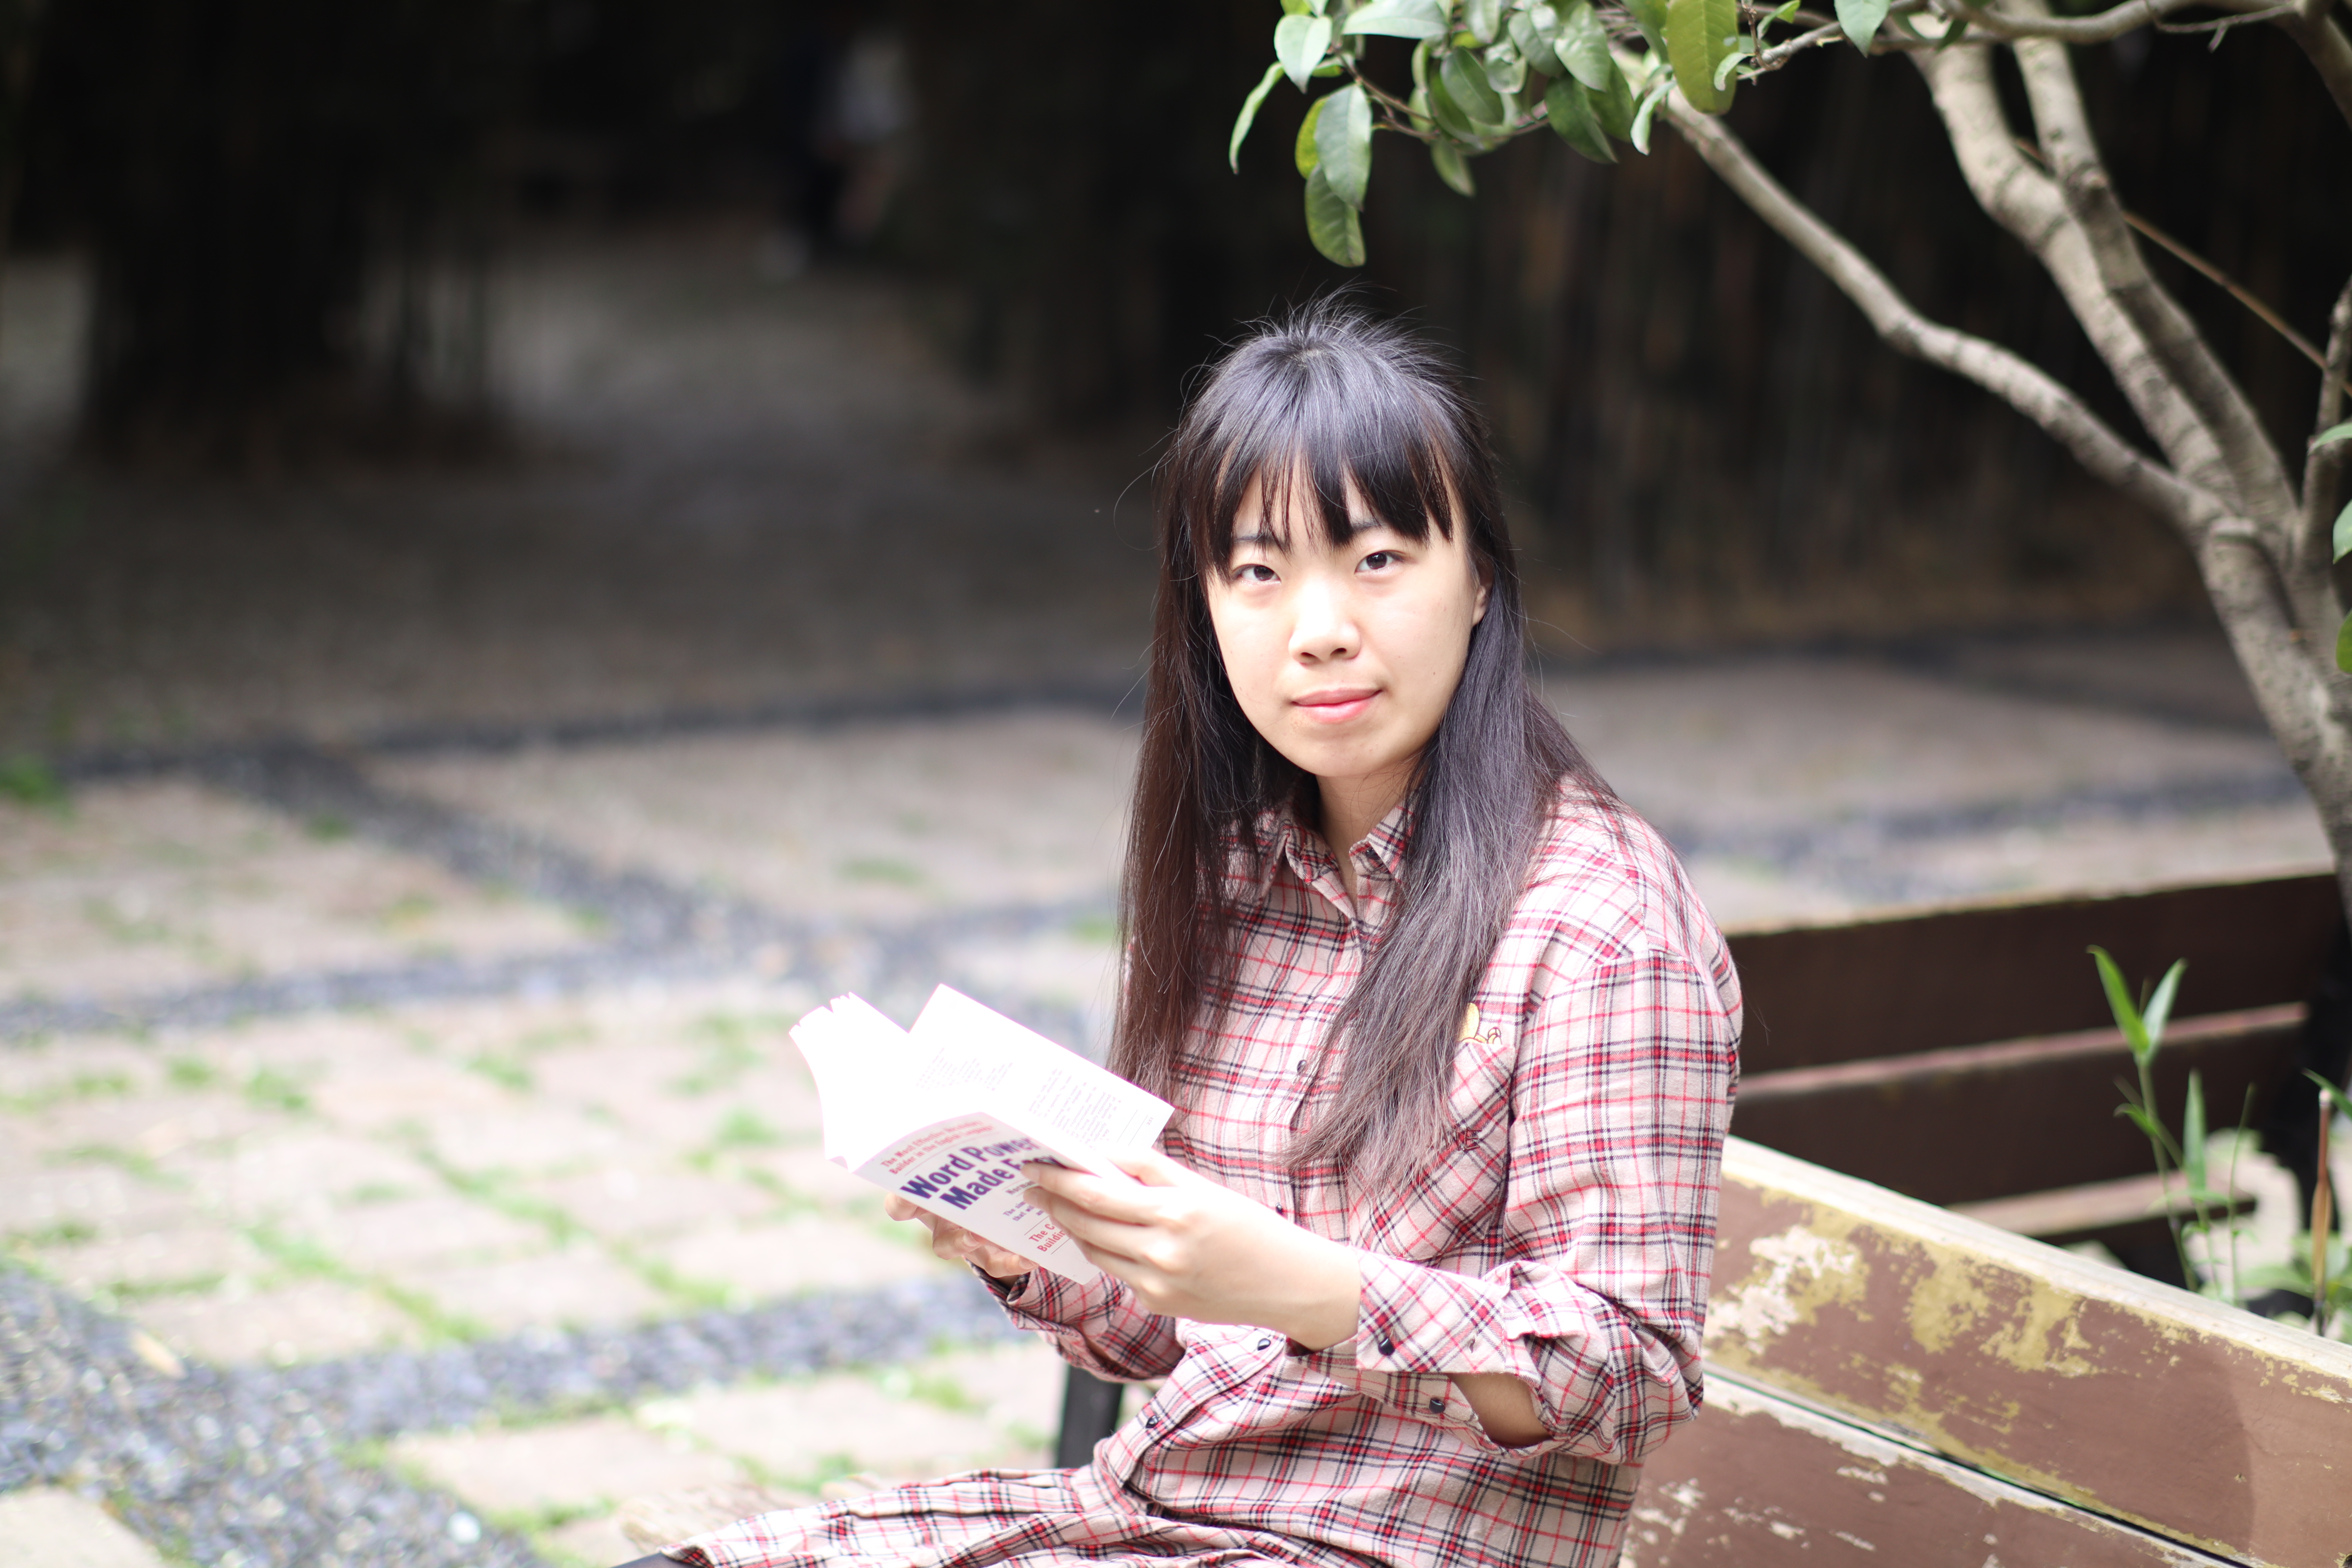
\includegraphics[width=0.8\textwidth]{F1}
    \caption{28mm f1.7 1/30 5500K}
    \label{F-02}
\end{figure}

上面的照片使用冷光LED灯作为光源拍摄,所摄物体为放置在木桌上的一张实验室的门禁卡。
该灯灯显色系数为97,可见色调与下面的照片有明显不同。

\section{所摄照片}
\begin{figure}[H]
    \centering
    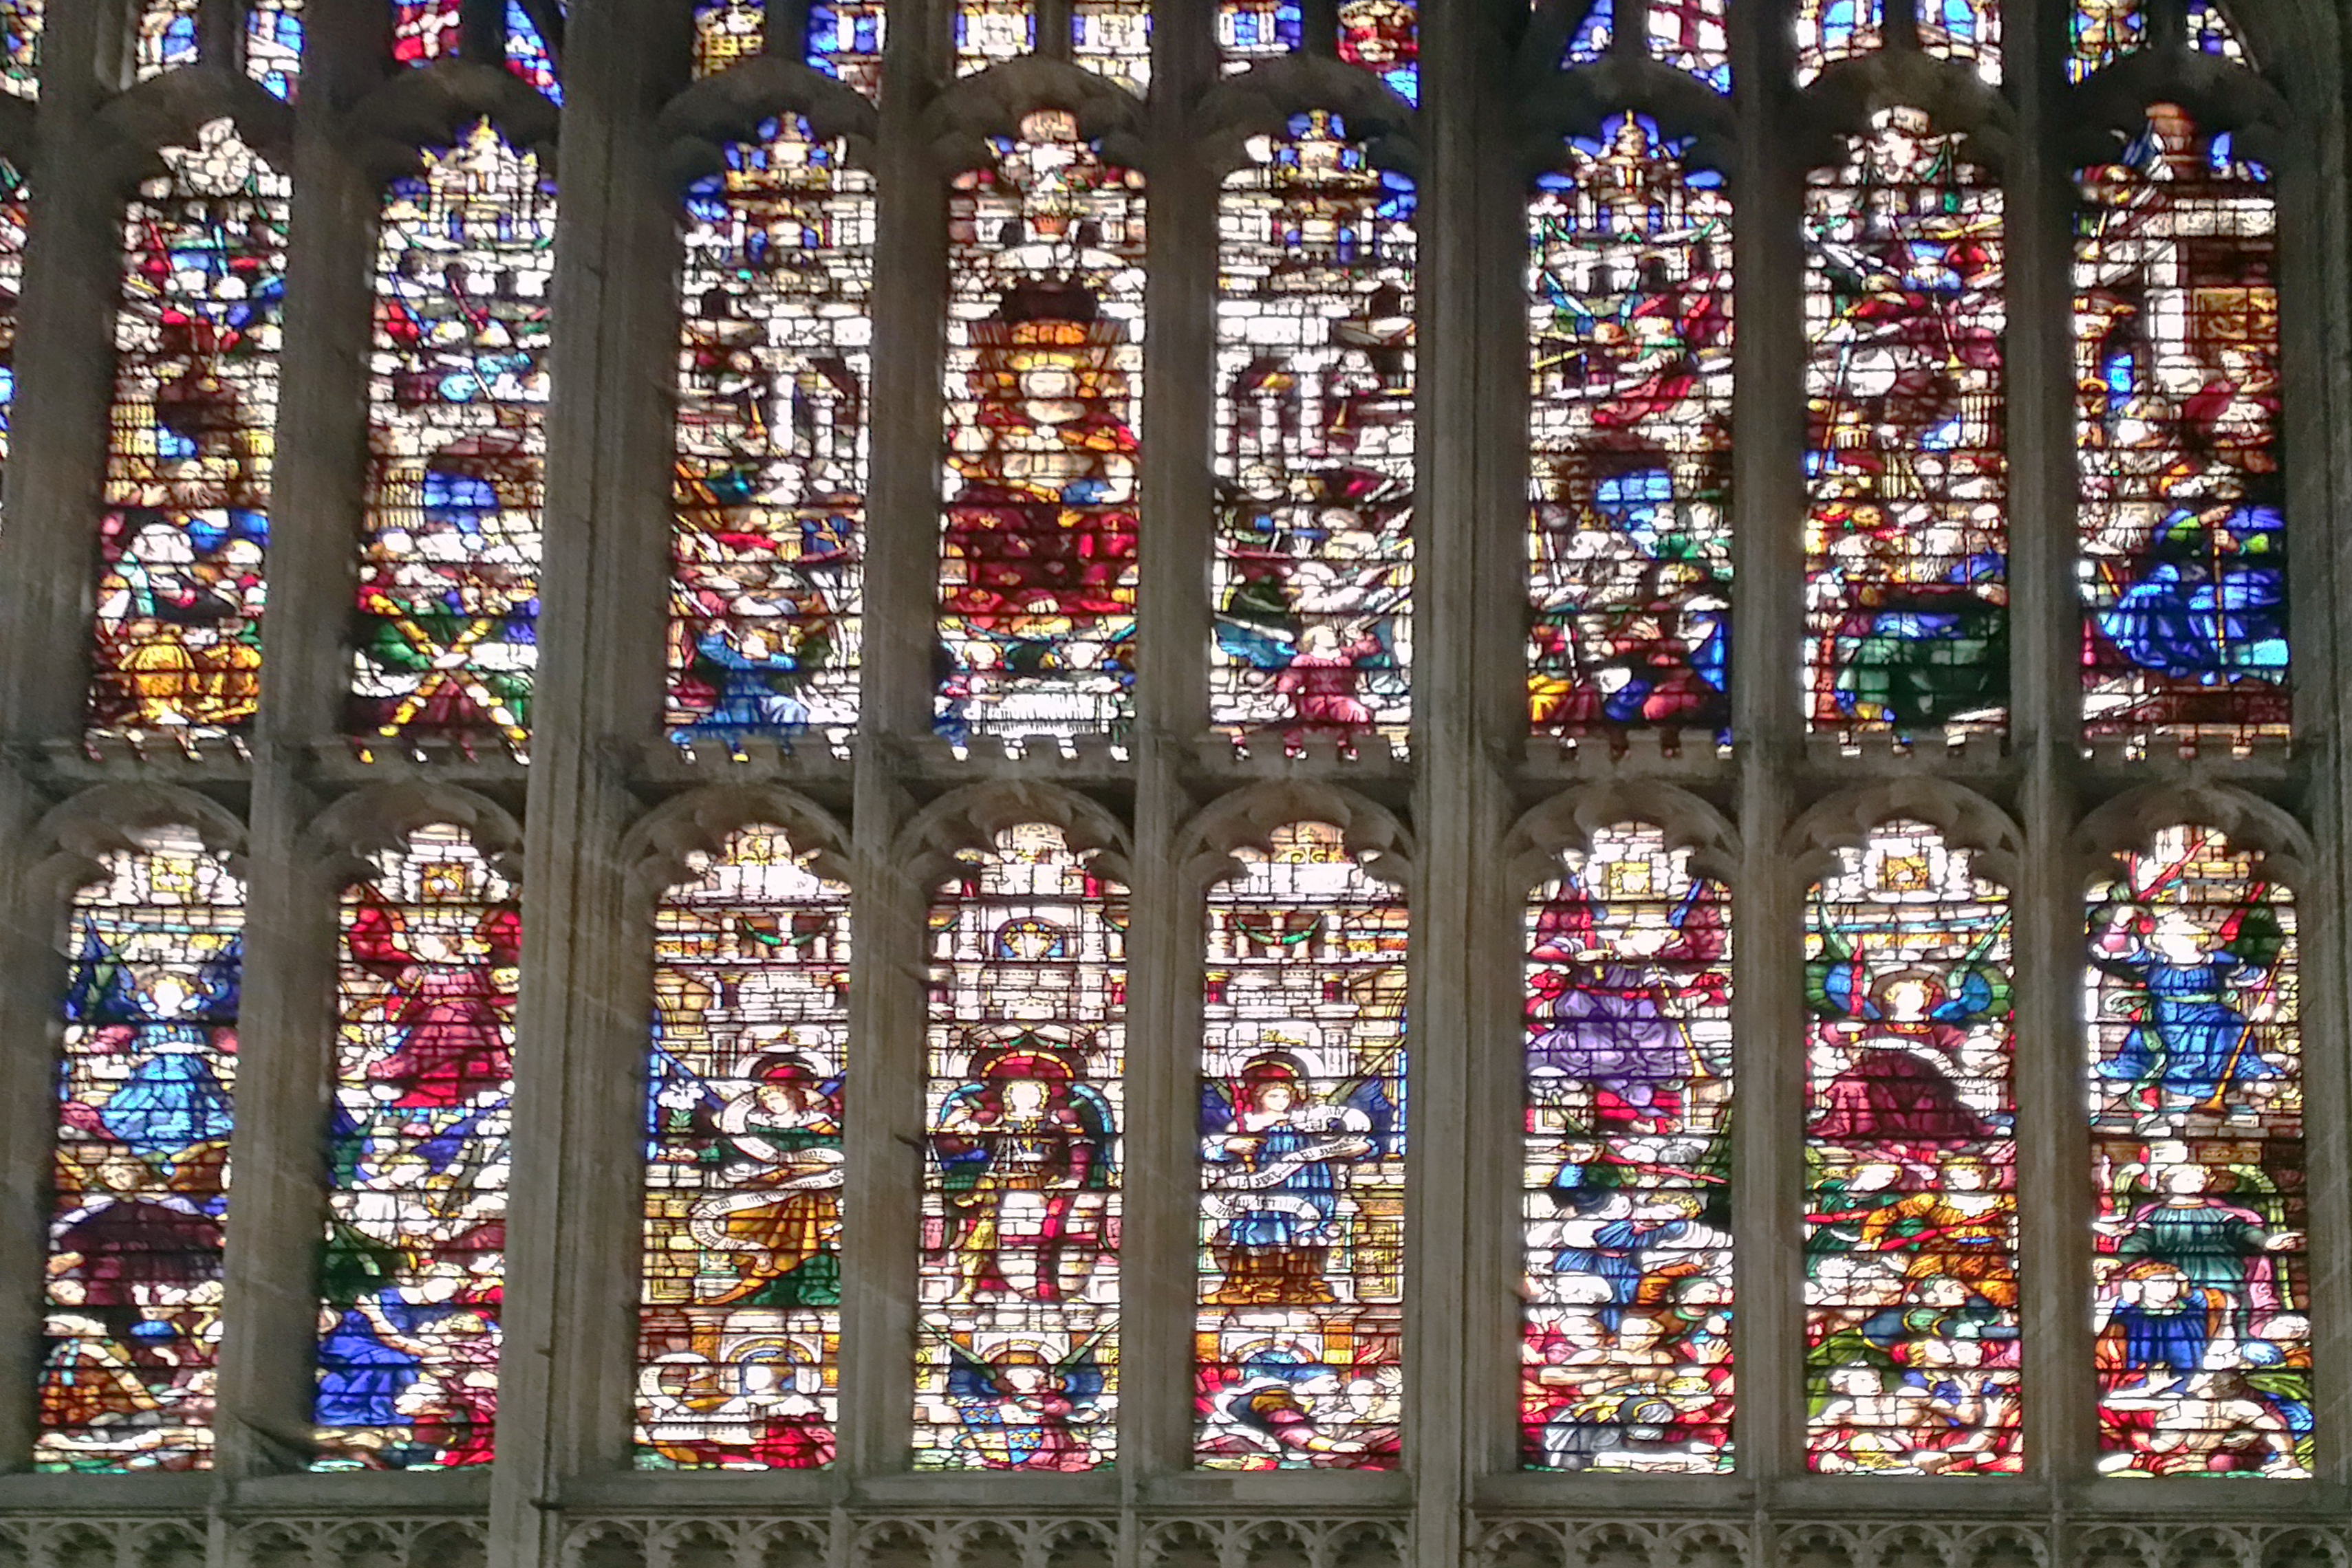
\includegraphics[width=0.9\textwidth,angle=0]{F2}
    \caption{28mm f1.7 1/30 3000K}
    \label{F-01}
\end{figure}

上面的照片使用暖光LED灯作为光源拍摄,该灯灯显色系数为97,可见色调与上面的照片有明显不同。

%\bibstyle{unsrt}
%\bibliography{references}{}
\end{document}
